
\documentclass{beamer}

\usepackage{bbm}
\usepackage{amsmath}

\newcommand{\argmax}{\operatornamewithlimits{argmax}}

% There are many different themes available for Beamer. A comprehensive
% list with examples is given here:
% http://deic.uab.es/~iblanes/beamer_gallery/index_by_theme.html
% You can uncomment the themes below if you would like to use a different
% one:
%\usetheme{AnnArbor}
%\usetheme{Antibes}
%\usetheme{Bergen}
%\usetheme{Berkeley}
%\usetheme{Berlin}
%\usetheme{Boadilla}
%\usetheme{boxes}
%\usetheme{CambridgeUS}
%\usetheme{Copenhagen}
\usetheme{Darmstadt}
%\usetheme{default}
%\usetheme{Frankfurt}
%\usetheme{Goettingen}
%\usetheme{Hannover}
%\usetheme{Ilmenau}
%\usetheme{JuanLesPins}
%\usetheme{Luebeck}
%\usetheme{Madrid}
%\usetheme{Malmoe}
%\usetheme{Marburg}
%\usetheme{Montpellier}
%\usetheme{PaloAlto}
%\usetheme{Pittsburgh}
%\usetheme{Rochester}
%\usetheme{Singapore}
%\usetheme{Szeged}
%\usetheme{Warsaw}



\title{Portfolio Playground}

% A subtitle is optional and this may be deleted
\subtitle{CPSC 437/537}

\author{Chris Harshaw \\ Daniel Keller \\ Felipe Pires}

\date{\today}
% - Either use conference name or its abbreviation.
% - Not really informative to the audience, more for people (including
%   yourself) who are reading the slides online

% If you have a file called "university-logo-filename.xxx", where xxx
% is a graphic format that can be processed by latex or pdflatex,
% resp., then you can add a logo as follows:

% \pgfdeclareimage[height=0.5cm]{university-logo}{university-logo-filename}
% \logo{\pgfuseimage{university-logo}}

% Delete this, if you do not want the table of contents to pop up at
% the beginning of each subsection:
\AtBeginSubsection[]
{
  \begin{frame}<beamer>{Outline}
    \tableofcontents[currentsection,currentsubsection]
  \end{frame}
}

% Let's get started
\begin{document}

\begin{frame}
  \titlepage
\end{frame}

\section*{Motivation}
\begin{frame}{Motivation}
\centering
We've \textbf{all} wanted to trade stocks 

\pause

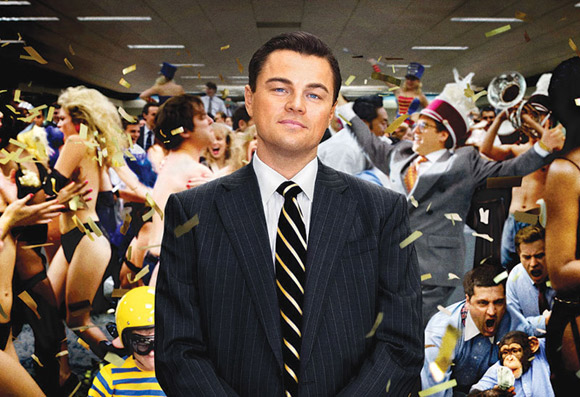
\includegraphics[width=0.5\textwidth]{wallstreet_2}

\pause

...but are afraid to lose large amounts of money

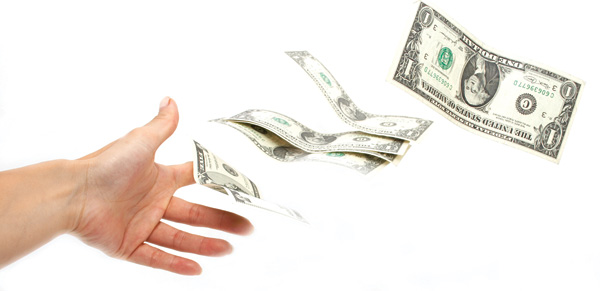
\includegraphics[width=0.5\textwidth]{lose_money}
  
\end{frame}

\begin{frame}{Motivation}
\textbf{Solution:} \emph{Paper Trading} -  simulated trading to practice buying and selling securities without actual money being involved.

\begin{center}
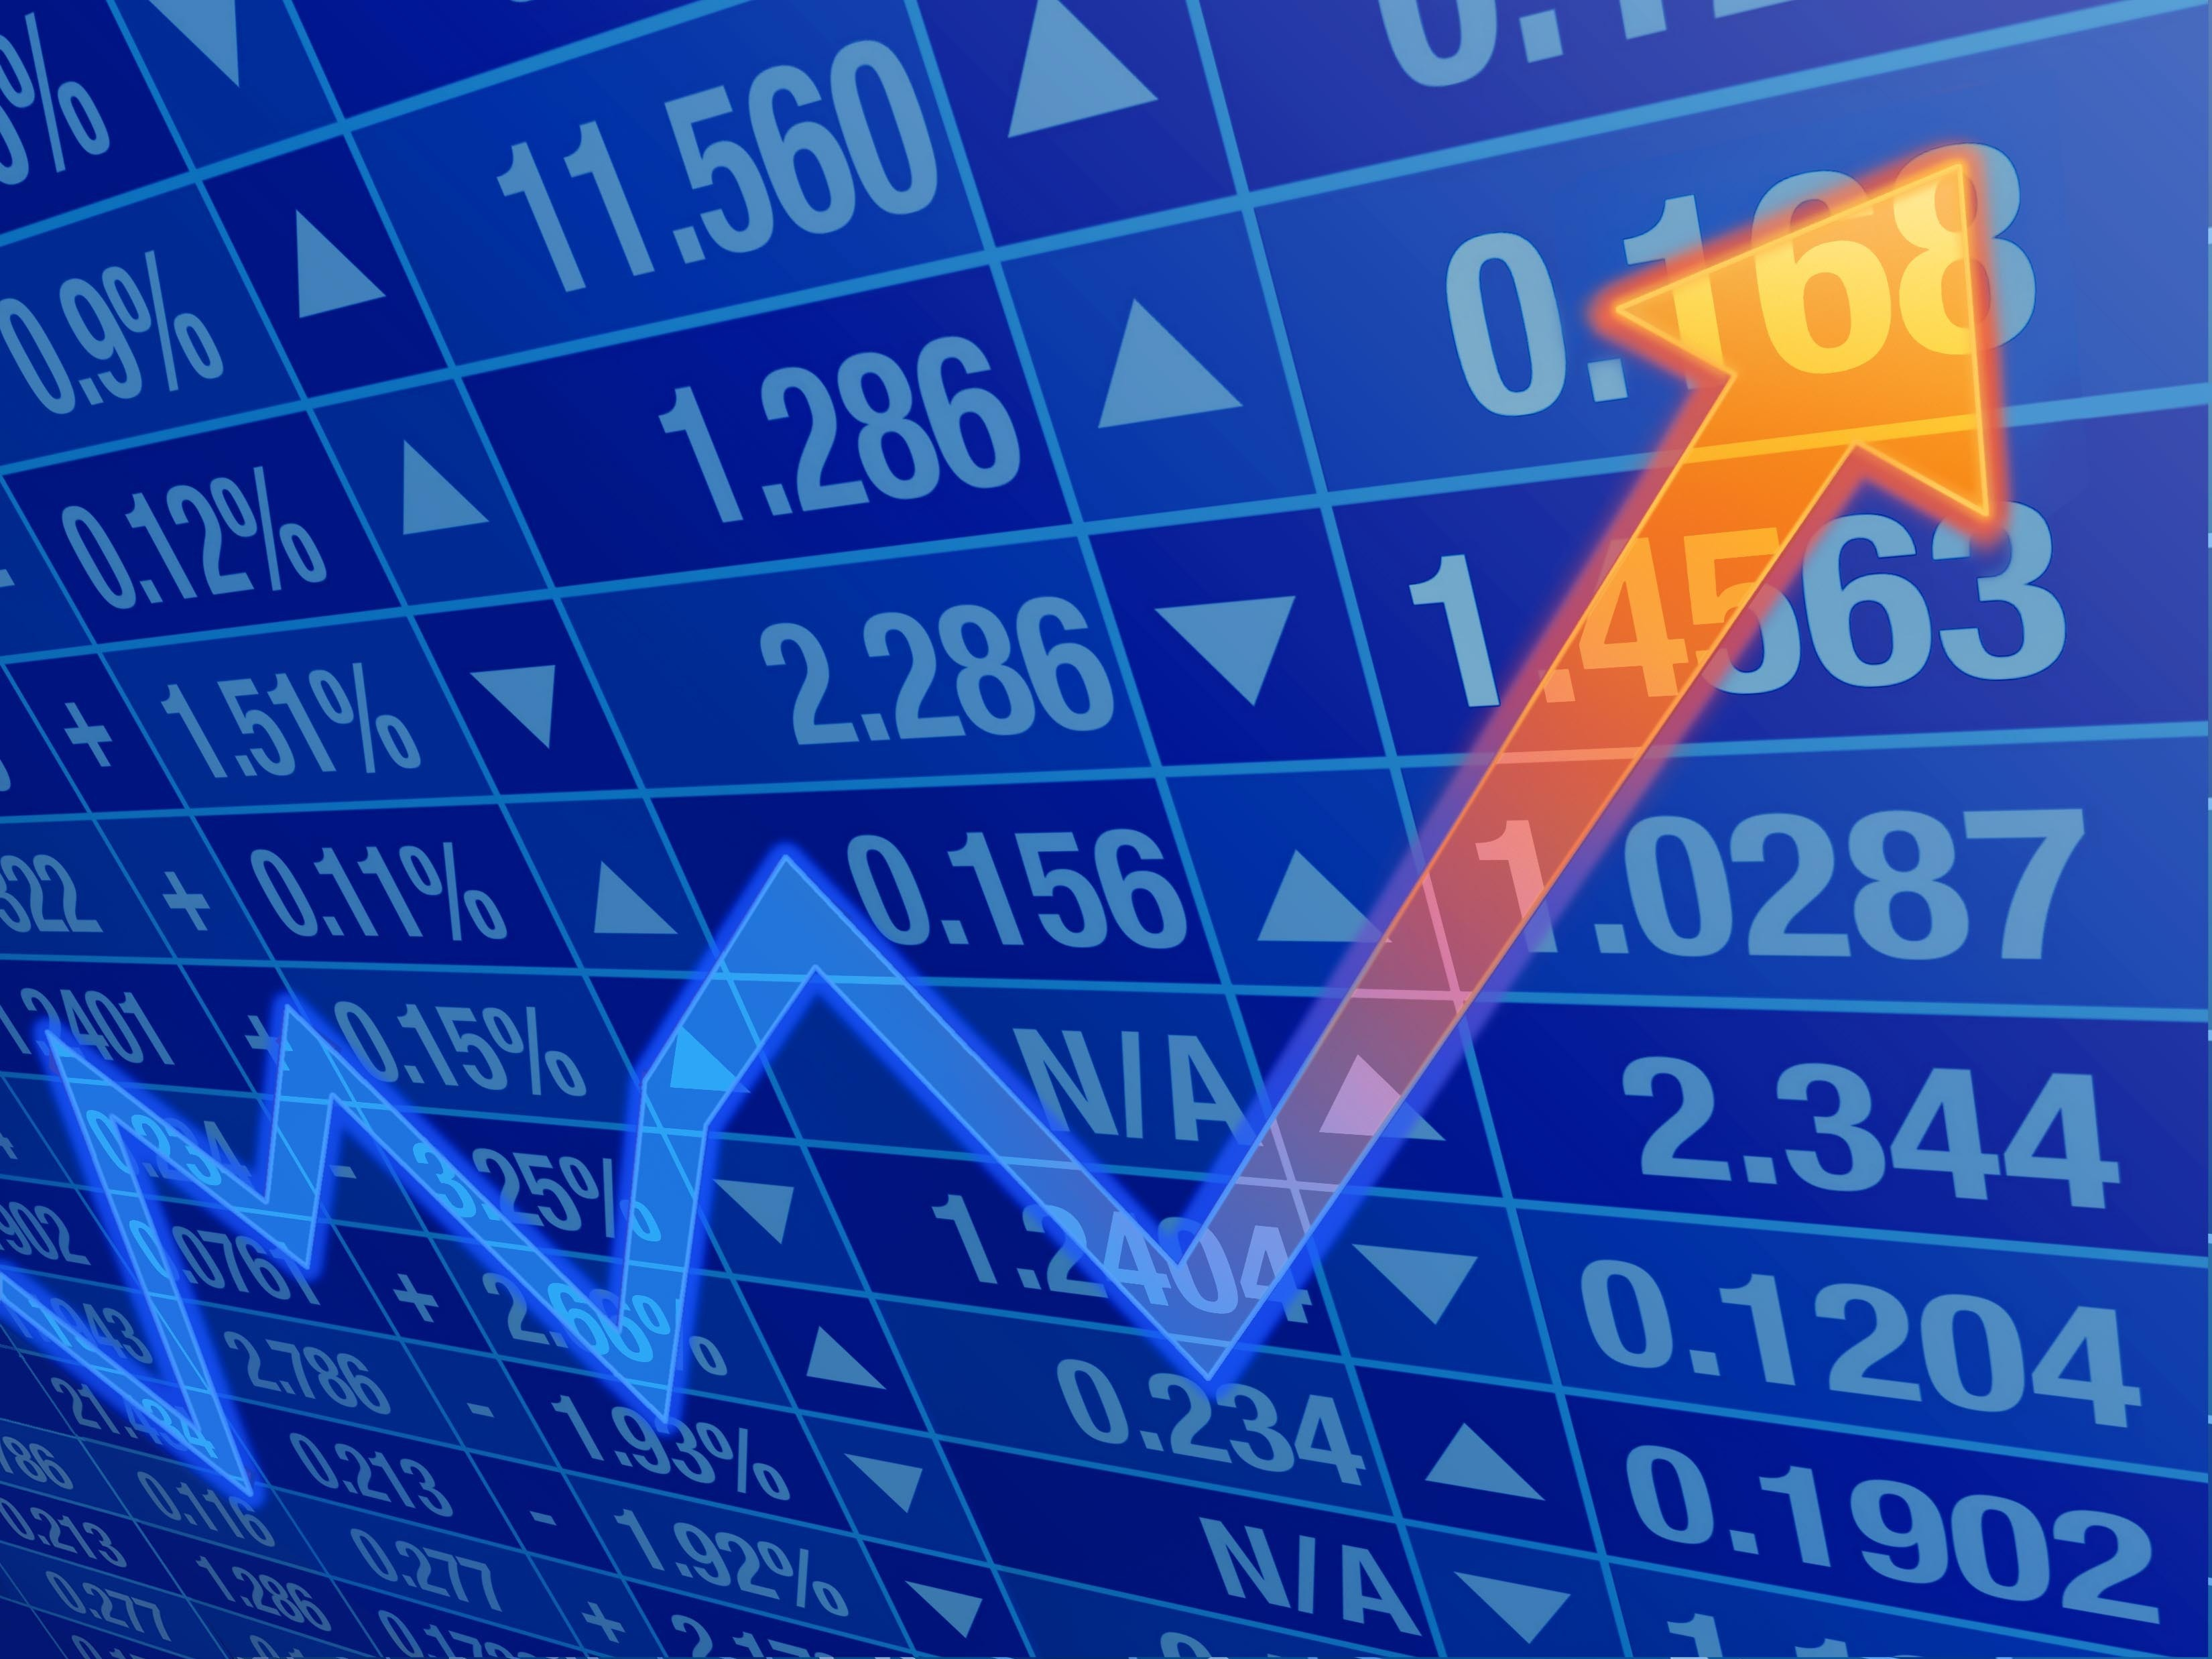
\includegraphics[width=0.5\textwidth]{stock_stock}
\end{center}

\pause

Enter \textbf{\textcolor{blue}{ Portfolio Playground}}, the premier paper-trading web application developed at Yale University!


  
\end{frame}

\begin{frame}{Outline}
  \tableofcontents
  % You might wish to add the option [pausesections]
\end{frame}

% Section and subsections will appear in the presentation overview
% and table of contents.
\section{Main Functionality}

\begin{frame}{Main Functionality}
Portfolio Playground is a paper trading web-application with three main functionalities \\

	\begin{itemize}
		\item Portfolio creation and analysis
		\item Portfolio comparison
		\item Portfolio recommendation
	\end{itemize}

\end{frame}

\begin{frame}{Main Functionality - Creation and Analysis}
FRONT END PICTURE GOES HERE

Our portfolio creation supports a variety of features including
	\begin{itemize}
		\item Stocks pulled from over 37,000 US equities and mutual funds
		\item Large amounts of historical stock price data (19XX-2016)
		\item User inputs include number of shares purchased, portfolio creation date
	\end{itemize}
\end{frame}

\begin{frame}{Main Functionality - Creation and Analysis}

Suppose we have a portfolio $P$ consisting of stocks $P = \{s_1\dots s_N\}$, where $x_i$ is the number of shares of stock $s_i$, $D_i$ is the dividends for stock $s_i$, and $P^{t}_{i}$ is the price of a single share of stock $s_i$ at time $t$. Then we can define,

\begin{block}{Total Stock Return - (Weighted Percent Increase)}
$$TSR = \sum_{i=1}^N x_i \left( \frac{P^{t_f}_{i} - P^{t_0}_{i} + D_i}{P^{t_0}_{i}} \right) $$
\end{block}

\begin{block}{Diversity - (Weighted Correlation Coefficients)}
$$Div = 1 - \frac{1}{Z} \sum_{i<j}^N x_i x_j Cor(P_i,P_j) \in \left[ 0,1 \right]$$ 
\end{block}

\end{frame}

\begin{frame}{Main Functionality - Comparison}
FRONT END PICTURE GOES HERE

Our portfolio comparison supports a variety of features including
	\begin{itemize}
		\item Stock price, total stock return, and diversity comparisons
		\item Aesthetically pleasing visualizations
	\end{itemize}

\end{frame}

\begin{frame}{Main Functionality - Recommendation}
The most unique feature of Portfolio Playground is its state-of-the-art recommendation algorithms. This helps shape trading intuition for novice traders. The algorithms used are

\begin{itemize}
\item Random
\item Highest Return
\item Diverse Options
\end{itemize}

\end{frame}

\section{Recommender Algorithms}
\begin{frame}{Recommender Algorithms - Random}
The Random algorithm recommends a random portfolio under a total budget constraint.

\begin{block}{Highest Return}
\begin{enumerate}
	\item Initialize portfolio $P = \emptyset$. Until budget constraints active,
		\begin{enumerate}
			\item $P \leftarrow P +$ random stock, random number of shares (under budget constraint)
		\end{enumerate}
\end{enumerate}
\end{block}

\pause
This can be used as a ``control portfolio'' and can also test the Efficient Market Hypothesis!
\end{frame}


\begin{frame}{Recommender Algorithms - Highest Return}
The Highest Return algorithm recommends an optimal forecasted portfolio under budget constraints such as total portfolio budget and maximum investment per stock.

\begin{block}{Highest Return}
\begin{enumerate}
	\item Fit a Vector Autoregression Model to historical stock data
	\item Forecast the stock prices $d$ days away
	\item Initialize portfolio $P = \emptyset$. Until budget constraints active,
		\begin{enumerate}
			\item $P \leftarrow P +$ stock that maximizes TSR
		\end{enumerate}
\end{enumerate}
\end{block}

\end{frame}

\begin{frame}{Recommender Algorithms - Diverse Options}
The Diverse Options algorithm recommends an optimal portfolio under budget constraints and \emph{diversity} or \emph{correlation} constraints.

\begin{block}{Diverse Options}
\begin{enumerate}
	\item Fit a Vector Autoregression Model to historical stock data
	\item Forecast the stock prices $d$ days away
	\item Initialize portfolio $P = \emptyset$. Until budget constraints active,
		\begin{enumerate}
			\item $A = \{s | corr(s,x) < \sigma \ \forall \ x \in P\}$ (options diverse from $P$)
			\item $P \leftarrow P +$ stock from $A$ that maximizes TSR
		\end{enumerate}
\end{enumerate}
\end{block}

\end{frame}

\section{Database Design}

\begin{frame}{Database Design}

What do we need to store?

Where are we getting it from?

\end{frame}


\begin{frame}{Database Design}

A diagram of the architecture goes here.

\end{frame}

\section{Front End Design}

\begin{frame}{Front End Design}

What are the design decisions?

\end{frame}

\begin{frame}{Front End Design}

What tools did we use to achieve this?

\end{frame}

\section*{Questions}
\begin{frame}{Questions}
\centering
Questions?
\end{frame}

\end{document}


